
%  ********************************************************************** 


\section{MECAGEN Model of Molecular and Genetic Regulation and Signaling}
%  ********************************************************************** 


The goal of this chapter is to briefly explain the principles of gene regulatory networks (GRNs), describe the components of GRN models, and give examples. In the present work, our particular objective was to design a simple and easily computable model of the molecular and genetic interactions that occur during development. This domain is a subject of intense research \cite{Wilczynski:2010jz}\cite{BenTaboudeLeon:2009vd}\cite{Giacomantonio:2010cl}, at the crossroads between bioinformatics, systems biology and chemical kinetics; nonetheless, we believe that relevant insight can already be gained by using simple rules. We articulate our model around three types of rules:
\begin{itemize}
	\item rules driving the dynamics of intracellular gene/protein reactions
	\item rules driving the dynamics of cellular secretion and transduction
	\item rules driving the dynamics of extracellular reactions, transport and diffusion
\end{itemize}

  These rules are expressed in a chemical kinetic framework by ODEs of the type $dp/dt=f(p,g,q,r)$, where $p$ represents protein concentrations, $g$ gene expression level, $q$ external ligands, and $r$ membrane receptors. Extracellular reactions, transport and diffusion of ligands are also taken into account via PDEs involving $\partial q/\partial t$ and fluxes $\vec{J}=-D\vec{\nabla}q$. 

To facilitate the specification of the parameters of molecular and genetic regulation, we interface the model with the BioTapestry software developed by W. Longabaugh and H. Bolouri at the Eric Davidson Lab, Caltech \cite{Longabaugh:2005bq}\cite{Longabaugh:2009kp} (Fig. \ref{model_grns_zebra_grn_yuh}). This software has been adopted by the developmental biology community as the standard tool to visualize gene regulatory networks. We use it to draw our own GRN and add different module parameters, then export it as an XML file used as an input into our model.
\begin{figure}
\begin{center}
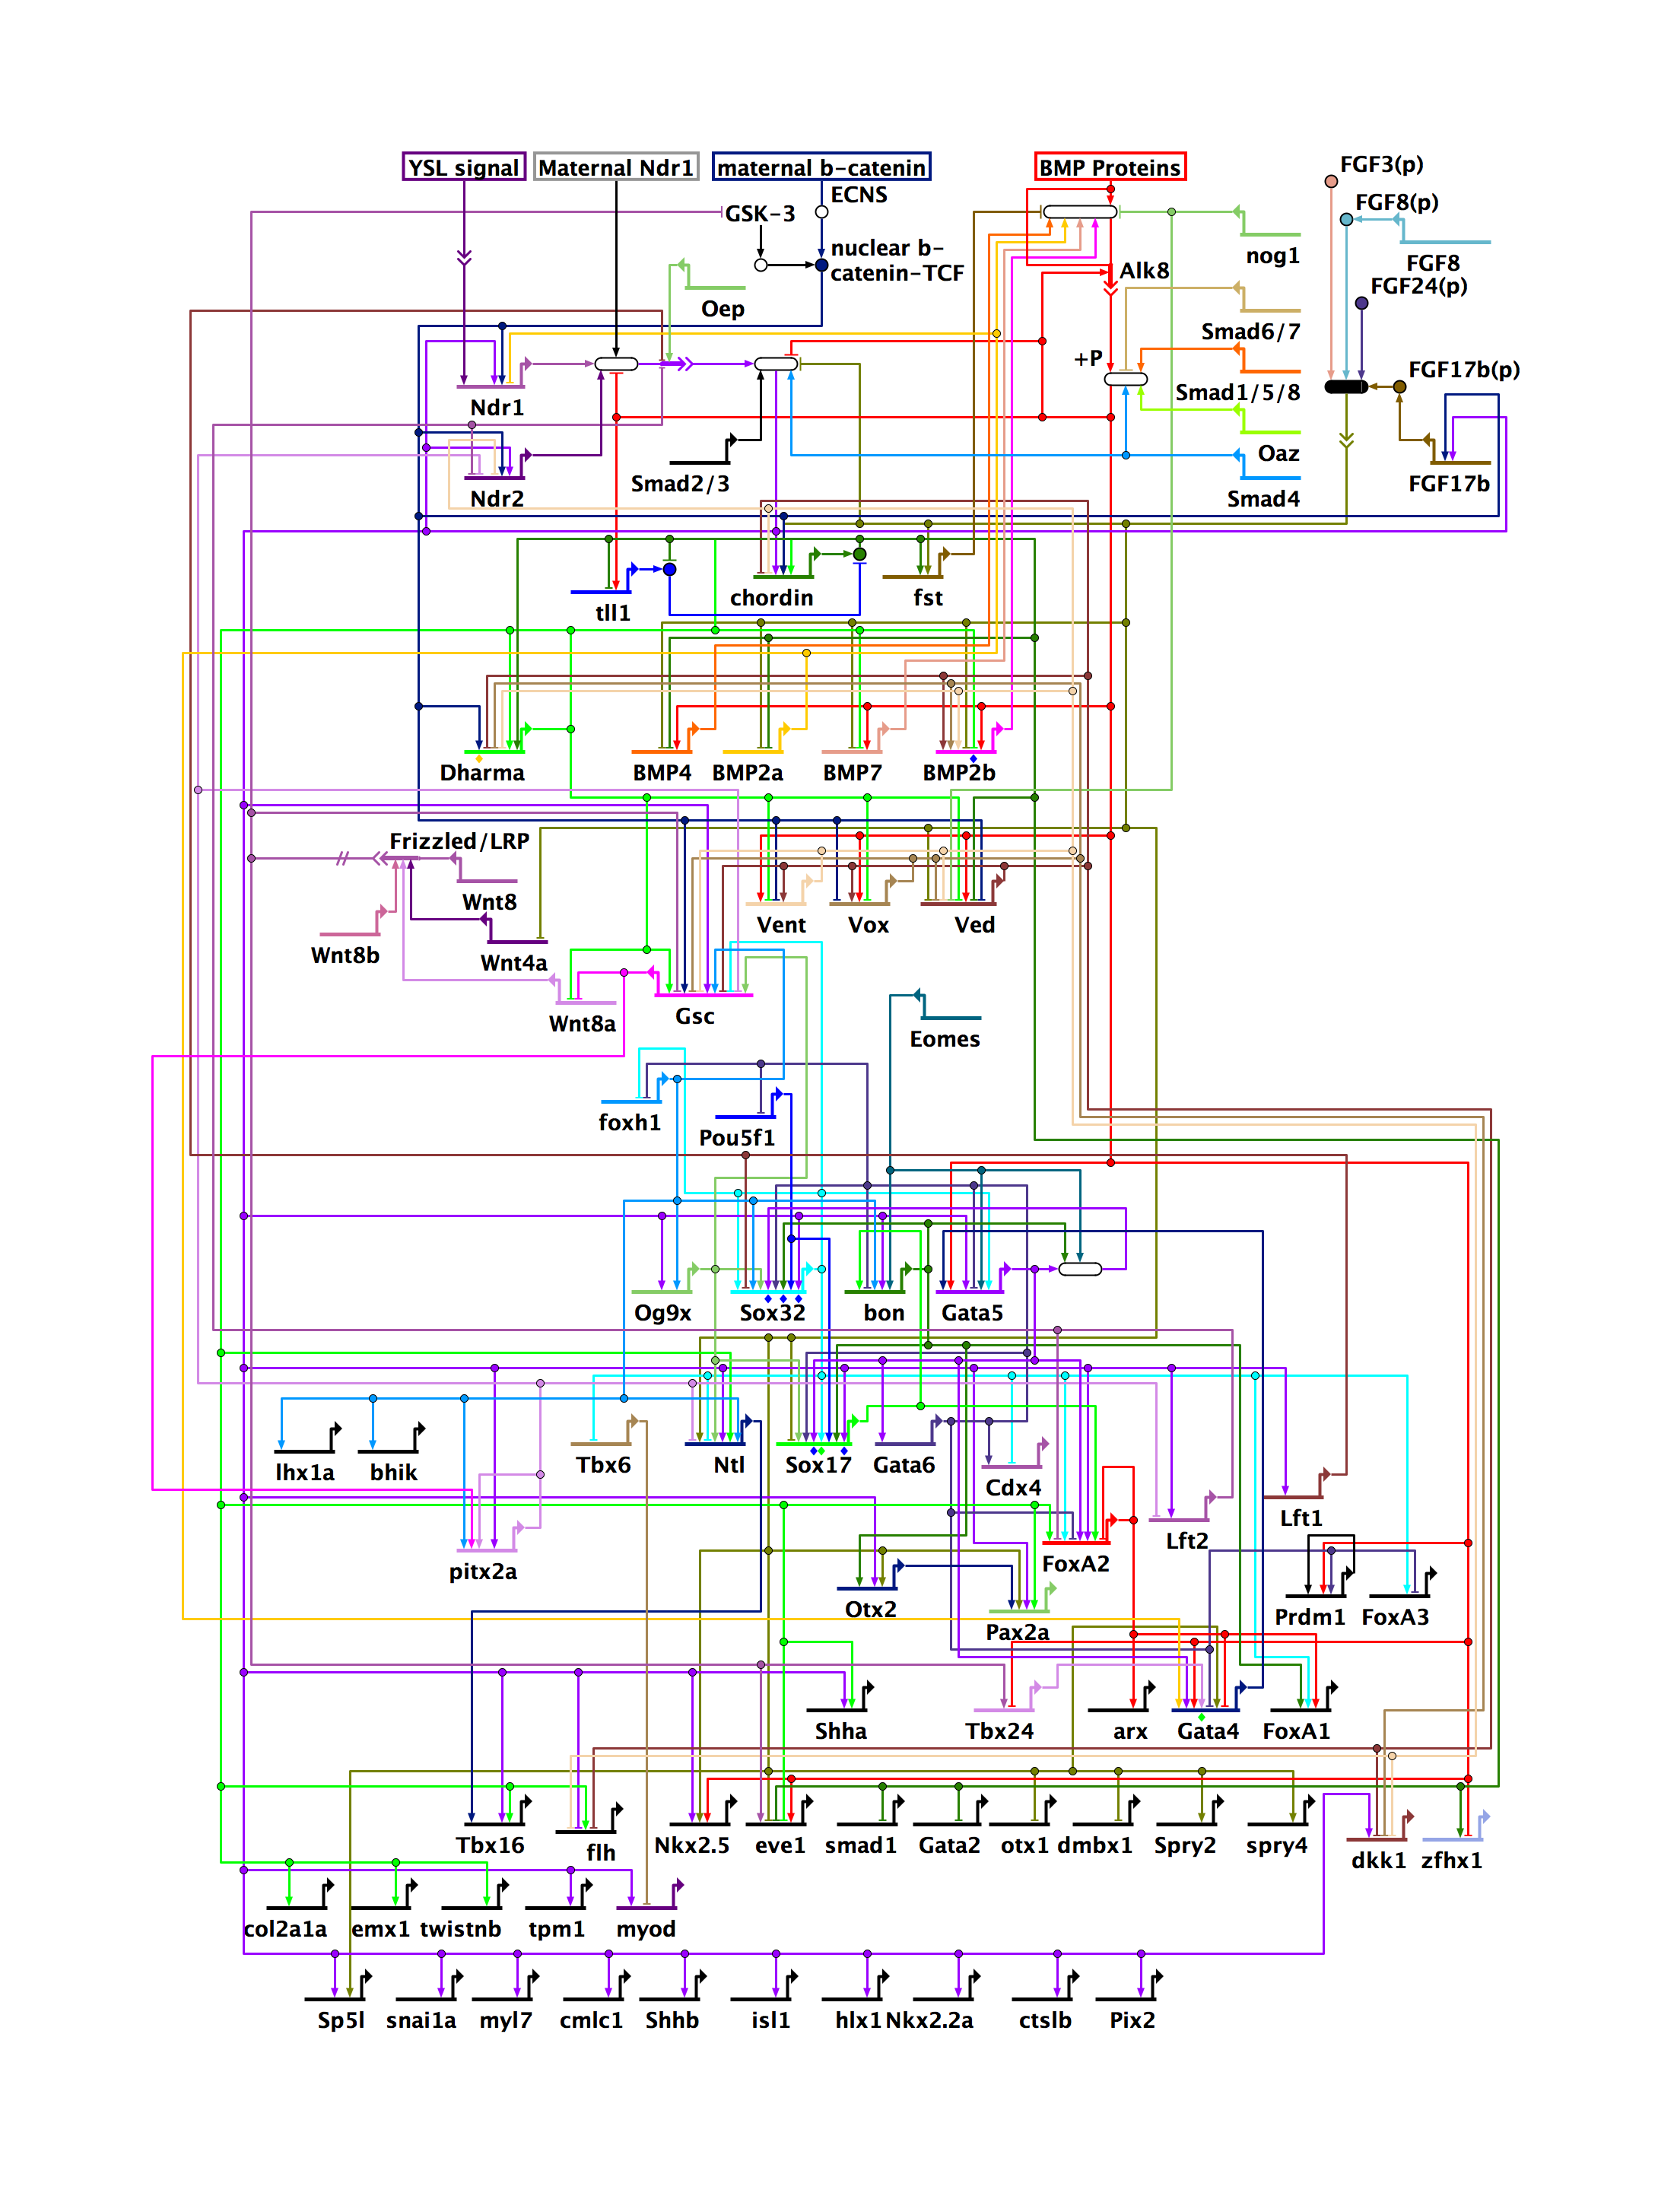
\includegraphics[width=0.6\textwidth]{../../images/model_grns/zebra_grn_yuh.png}
\end{center}
\caption{\textbf{BioTapestry representation of the developmental gene regulatory network (GRN) of the Zebrafish.} The network is presented in Chan et al., 2009 \cite{Chan:2009er}.}
\label{model_grns_zebra_grn_yuh}
\end{figure}
\begin{figure}
\begin{center}
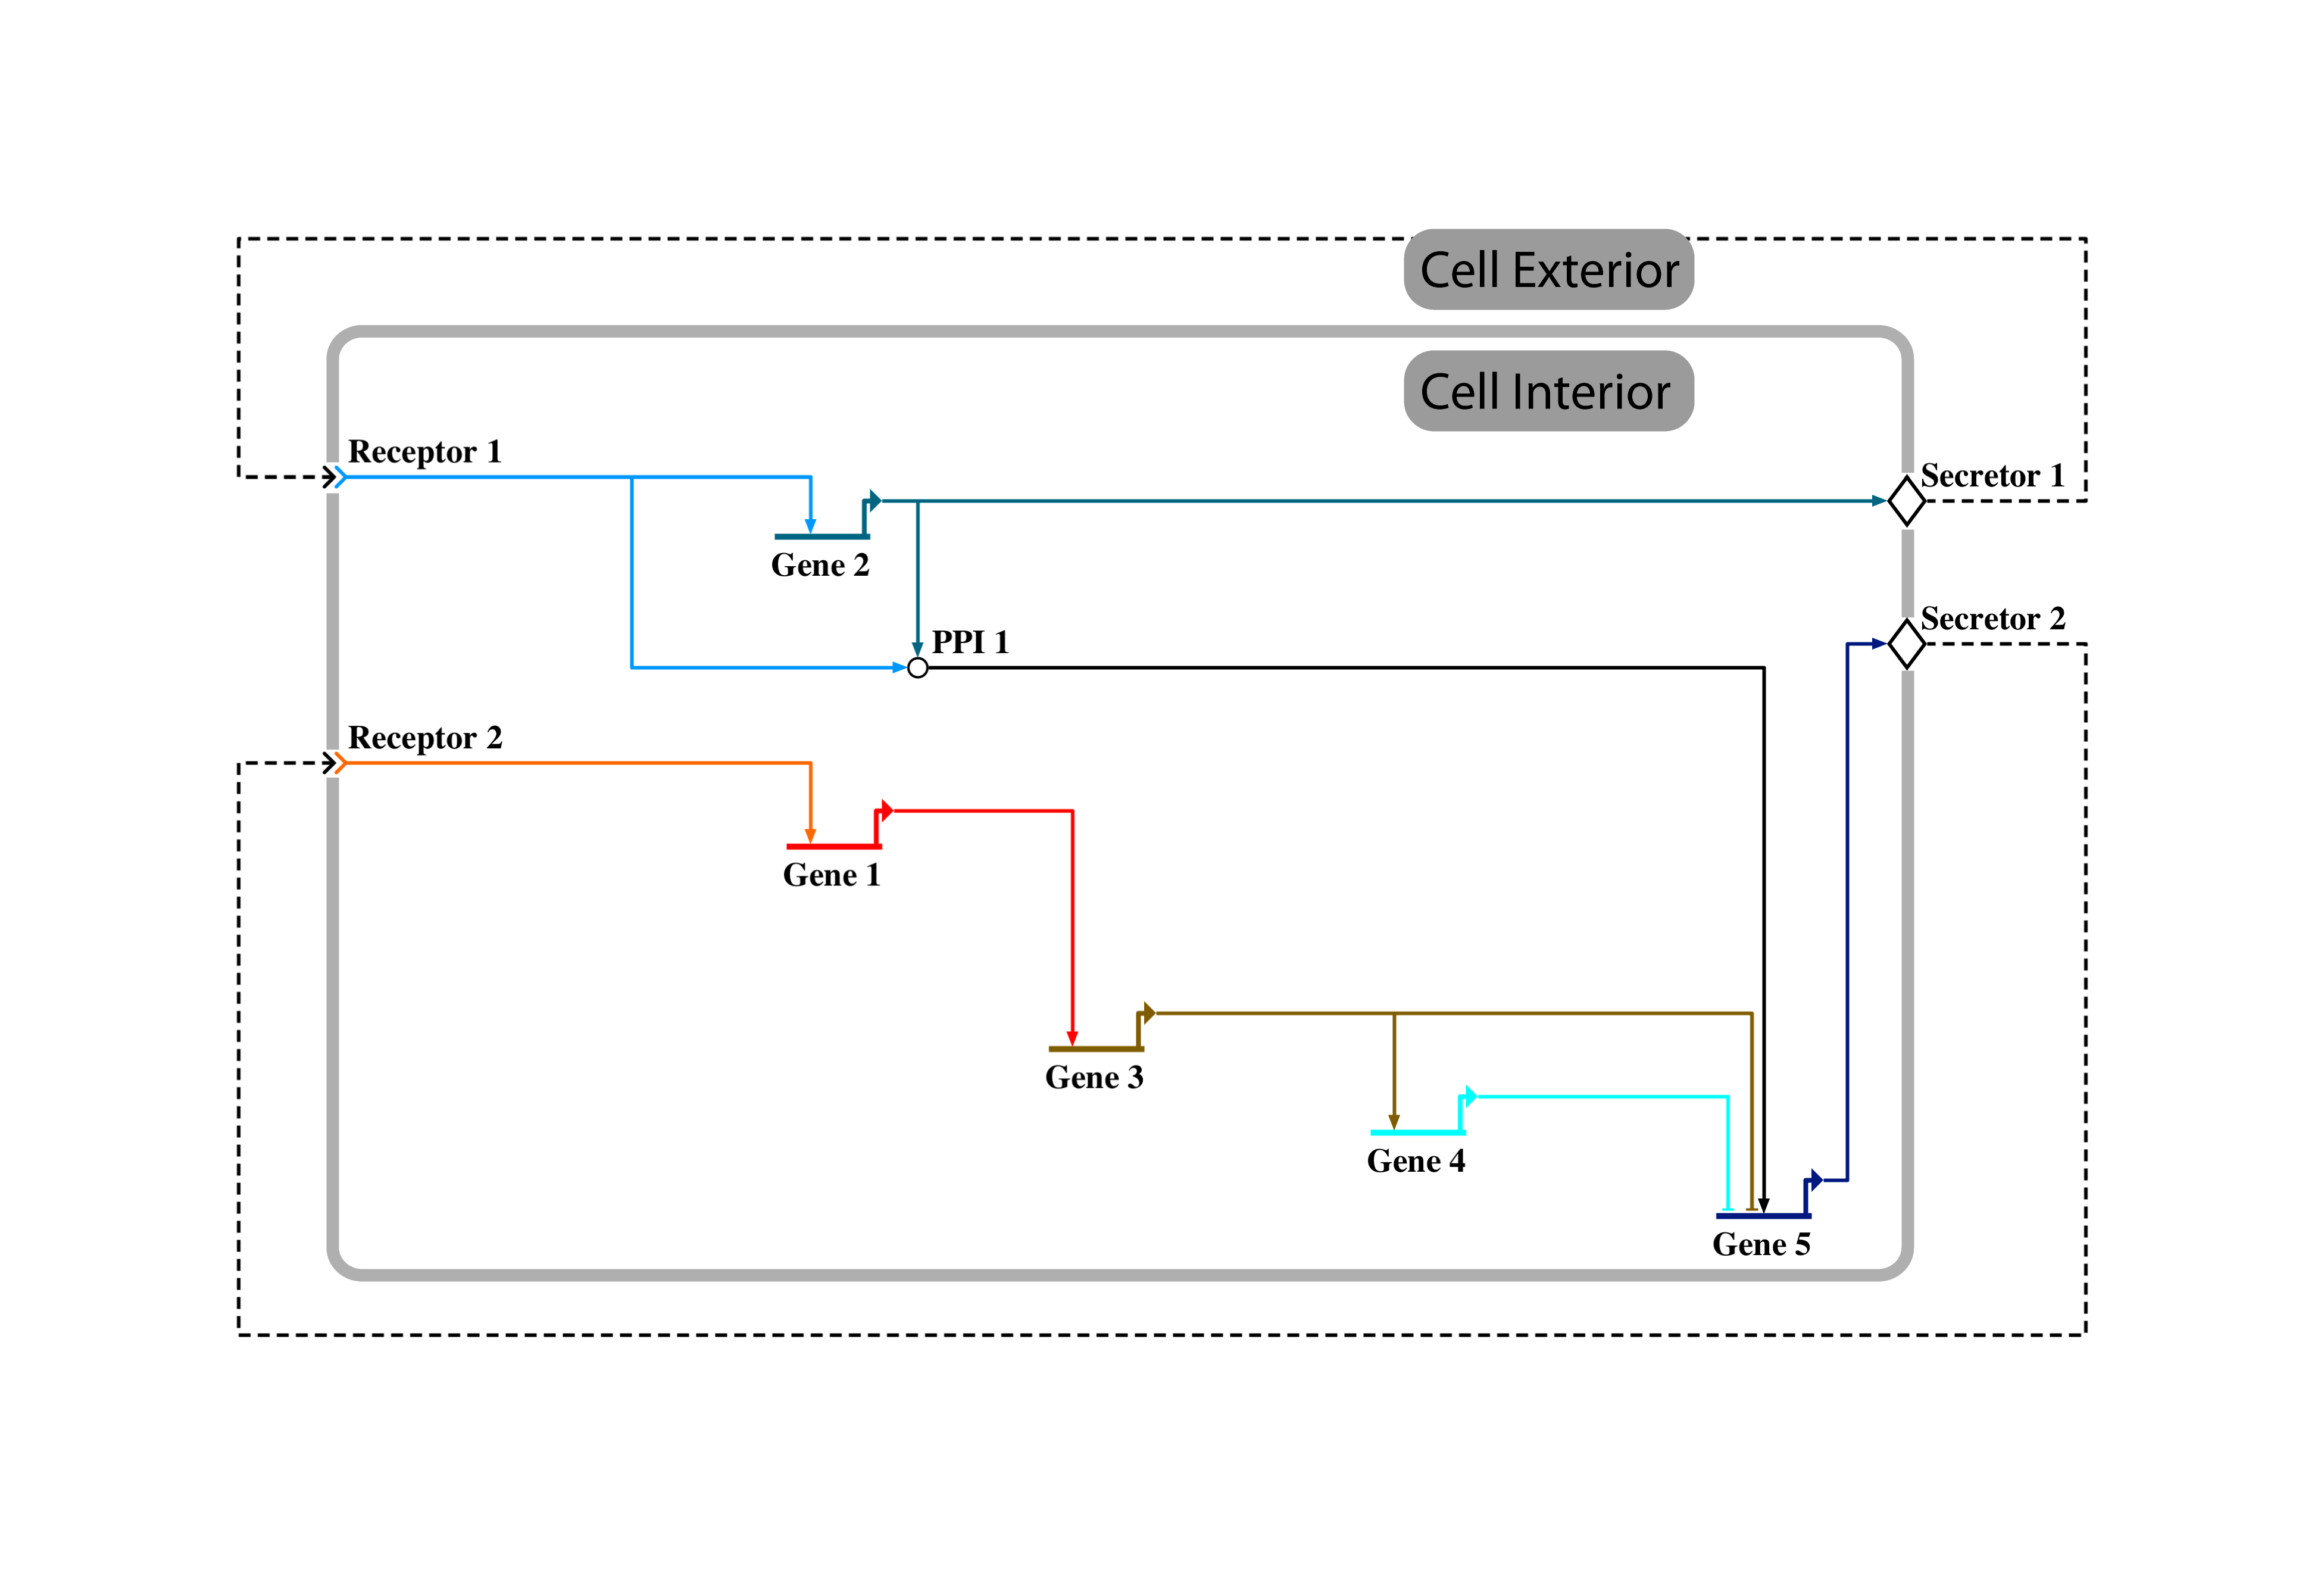
\includegraphics[width=0.9\textwidth]{../../images/Cases_Studies/Case_theo_grn/generic_grn_cellshape.png}
\end{center}
\caption{\textbf{Abstract gene regulatory network (GRN) produced by the BioTapestry software.} This GRN introduces the components integrated in the MECAGEN model of molecular and genetic regulation and signaling: protein-protein interactions (PPI), genes and their cis-regulatory elements (Gene), signal secretion module (Secretor), signal transduction module (Receptor). The arrows comprised in the cell interior represent intracellular proteins and the dashed arrows represent the extracellular ligand. Practically, the topology and the parameters of the GRN are specified by the user in BioTapestry, then a xml file is saved and it will serve as an input in of the MECAGEN model. Solid lines represent intra-cellular proteins and dashed lines represent extra-cellular ligands.}
\label{Case_theo_grn_generic_grn_cell_shape}
\end{figure}
\begin{figure}
\begin{center}
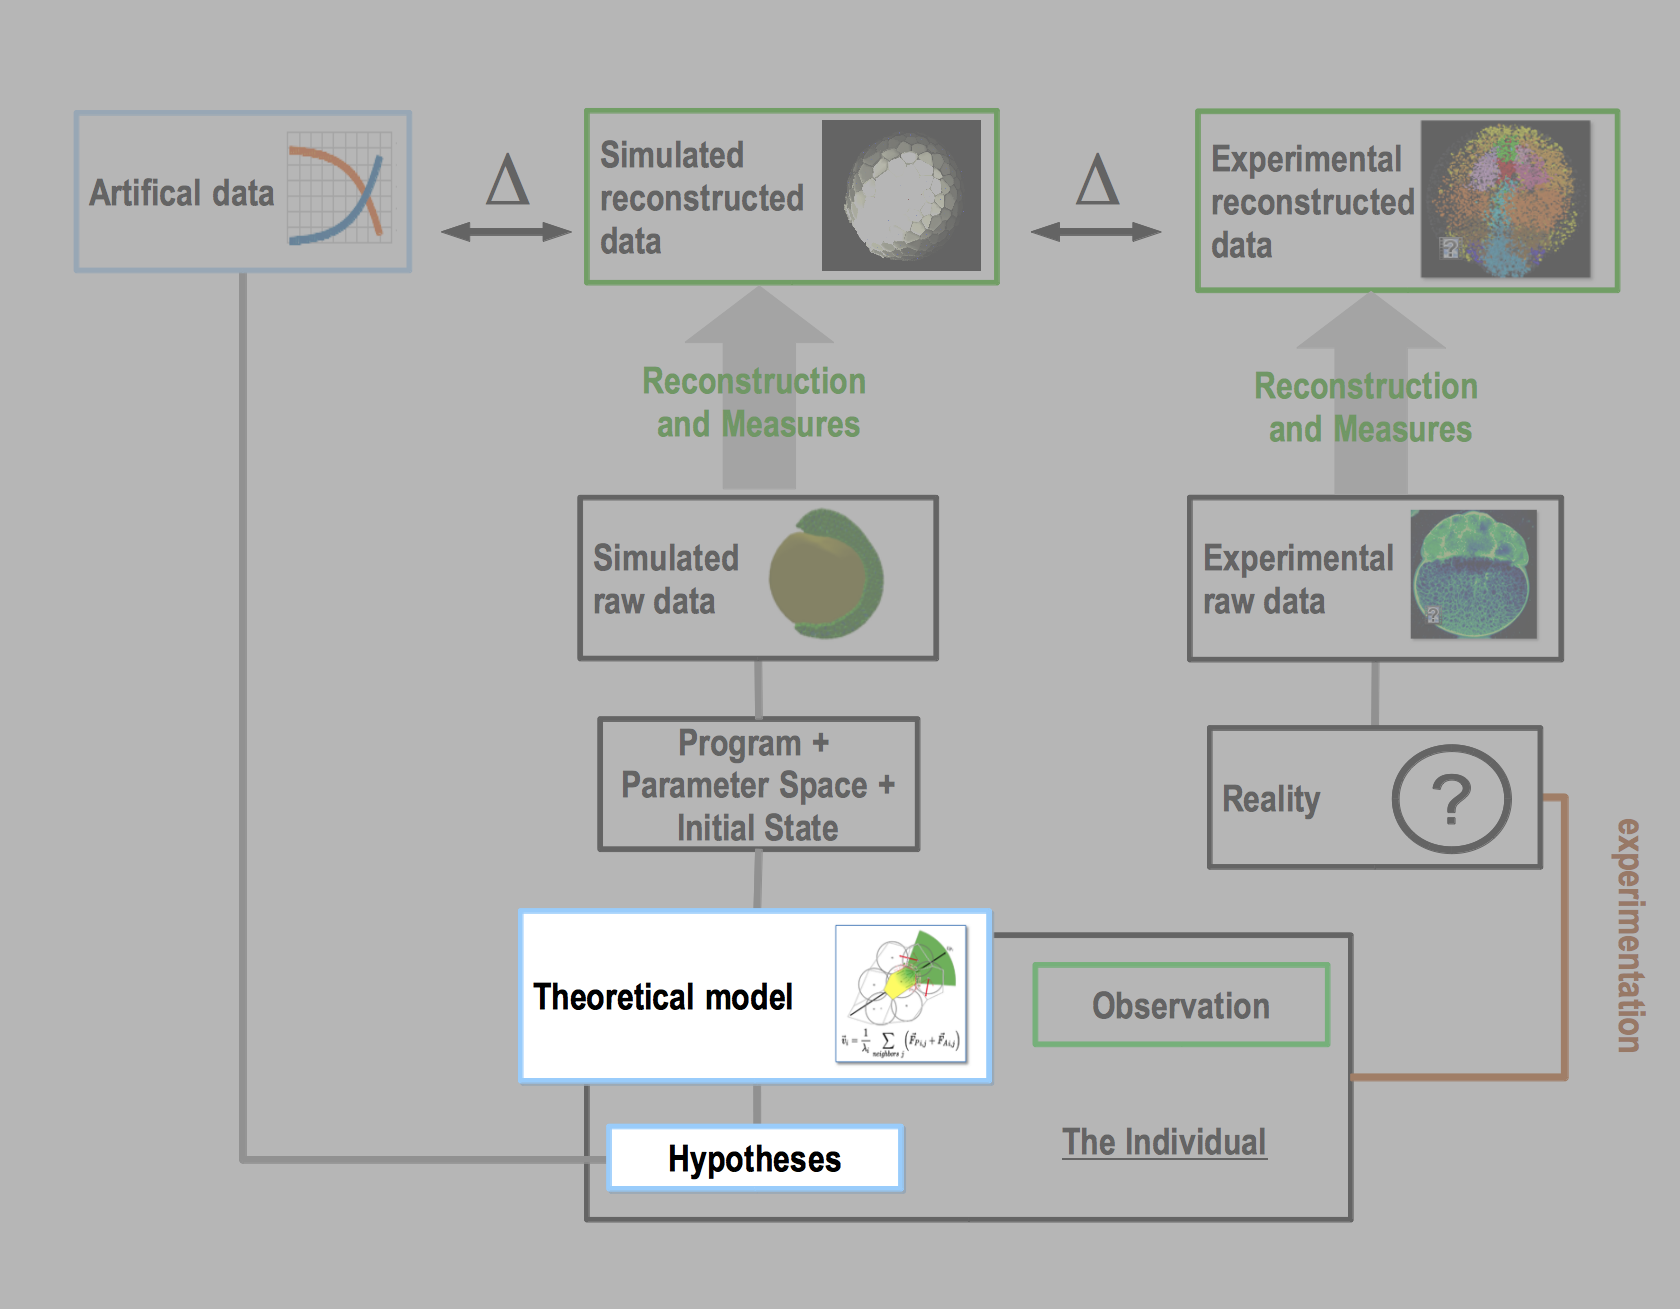
\includegraphics[width=0.75\textwidth]{../../images/experimental_science/experimental_science_cleaner_focus_theo.png}
\end{center}
\caption{\textbf{Situation of Chapter 4 in the methodological workflow.}}
\label{experimental_science_experimental_science_cleaner_focus_theo_2}
\end{figure}
%  ====================================================================== 


\subsection{Intra-Cellular Gene/Protein Reactions}
%  ====================================================================== 


To simplify the interactions inside the cell, we restrict the variables to real-valued quantities $\mathbf{p}=\{p_a\}$ representing the different proteins $\{P_a\}$, with $a=0...N_p\!-\!1$, and binary states $\mathbf{g}=\{g_b\}$ representing the expression levels of genes $\{G_b\}$ involved in the GRN, with $b=0...N_g\!-\!1$. Note that $p_a$ can stand either for an actual "number" of molecules or for a "concentration" of molecule type (i.e. the number divided by the volume of the cell). This can be justified by assuming that every cell occupies about the same volume, and considering that the extracellular space also belong to the Voronoi territories of the cells (i.e. the abstract "borderline" between two cell territories runs along the middle of their interstitium).

The role of RNA is bypassed, as transcription and translation are merged into a single process. Thus in the following, the term "protein" denotes a unique molecule type synthesized by a corresponding gene, whether it is actually a protein or mRNA. Then, this "protein" may either react in a protein-protein interaction, or act as a transcription factor reacting on a gene regulatory element.

Here, each gene $G_b$ produces a single protein type $P_{a=b}$, but on the other hand there can be more protein types than genes (i.e. $N_g \leq N_p$) because the GRN model covers only a small part of the whole genome and some proteins present in the cell can originate from extracellular signaling by neighboring cells. Proteins synthesized internally are in the same order as the genes in the interval $[0, N_g\!-\!1]$, then proteins of external origin are indexed in the interval $[N_g,N_p\!-\!1]$, if it is not empty. Protein concentrations $\mathbf{p}$ evolve according to three rules:
\begin{itemize}
	\item protein-protein interactions (first subsection below)
	\item synthesis by encoding genes (second subsection)
	\item degradation by the molecular environment (third subsection)
\end{itemize}

Gene activities are regulated by the proteins via Boolean functions representing a logical combination of promoters and repressors (fourth subsection).
%  ---------------------------------------------------------------------- 


\subsubsection{Protein-Protein Interactions}
%  ---------------------------------------------------------------------- 


Here we consider only protein-protein reactions involving two reactants and one product, generally expressed by:

$$\alpha_0 P_0 + \alpha_1 P_1 \overset{k}{\rightarrow} P_2$$

where $k$ is the rate coefficient. The corresponding rate equation reads:  

$$\frac{dp_2}{dt} = k\;p_0^{\alpha_0} p_1^{\alpha_1}$$

Further simplifying assumptions involve uniform stochiometric coefficients $\alpha_0 = \alpha_1 = 1$, and one of the two protein reactants in much greater concentration than the other, e.g. $p_0 \gg p_1$, in which case the rate equation boils down to a first-order type:

$$\frac{dp_2}{dt} = -\frac{dp_1}{dt} = k' p_1$$

where $k' = kp_0$ is the new "pseudo-coefficient" of the variation. Naturally, this very simple schema has important limitations. Yet, when applied to many nodes of a large network of molecular interactions inside each cell, and also combined with the other regulatory reactions described below and spatial diffusion by cell-to-cell signalling, it can already give rise to complex spatiotemporal dynamics in cellular tissue.
%  ---------------------------------------------------------------------- 


\subsubsection{Synthesis by Encoding Genes}
%  ---------------------------------------------------------------------- 


We assume here that if a gene $G_b$ is active, i.e. $g_b = 1$, the concentration $p_b$ of the protein $P_b$ that it encodes simply increases with a constant rate $\gamma_b$, which is characteristic of the gene:

$$\frac{dp_b}{dt} = \gamma_b g_b$$
%  ---------------------------------------------------------------------- 


\subsubsection{Degradation by the Molecular Environment}
%  ---------------------------------------------------------------------- 


In addition to specific protein-protein interactions and gene-to-protein synthesis, proteins $P_a$ are also degraded by various molecular elements present in the cell. We model this process by another simple equation, based on a constant degradation coefficient $\kappa_a$ characteristic of the protein:

$$\frac{dp_a}{dt} = -\kappa_a$$

Up to this point, combining the three laws above, the extended protein equations read:

$$\begin{cases}        \frac{dp_1}{dt} & = -k' p_1 + \gamma_1 g_1 - \kappa_1 \\[.5em]        \frac{dp_2}{dt} & = +k' p_1 + \gamma_2 g_2 - \kappa_2      \end{cases}$$

(assuming that they are both synthesized by genes, i.e. $N_g \geq 2$). In the sections below, we will add more terms coming from transduction and diffusion mechanisms, which represent the communication with the cell's exterior.  
%  ---------------------------------------------------------------------- 


\subsubsection{Cis-Regulatory Boolean Model of Gene Expression}
%  ---------------------------------------------------------------------- 


The activity of a gene $G_b$ is enhanced by the "presence" of certain promoting transcription factors (TFs, subsumed under the term "protein" here) and/or the "absence" of certain repressing TFs. Both types of TFs bind to the cis-regulatory sites of the gene, which are regions of the DNA near the gene sequence. As multiple TFs $P_a$ can potentially participate in the regulation of a cis-regulatory module $G_b$, something we denote by $P_a \curvearrowright G_b$, Boolean logic is a well-suited schematization of these interactions (\cite{Peter:2012dy}). To minimize the number of variables, we represent the potential participation of a TF combined with its effective presence/absence in a regulatory module by a unique matrix of Boolean variables $\mathbf{\Gamma}=\{\Gamma_{ab}\}$, which is globally indexed by $a=0...N_p\!-\!1$ and $b=0...N_g\!-\!1$, and depends on concentration levels $\mathbf{p}$:

$$\Gamma_{ab}(t) =   \begin{cases}     1 & \text{if}\;\; P_a \curvearrowright G_b \;\;\text{and}\;\; p_a(t) \geq \theta_{ab} \\[.5em]     0 & \text{if}\;\; P_a \curvearrowright G_b \;\;\text{and}\;\; p_a(t) \lt \theta_{ab}   \end{cases}$$

where the $\theta_{ab}$ parameters are concentration thresholds. The activity of gene $G_b$ is then determined by the Boolean output of a logic function $f_b$, which is a combination of the Boolean operators AND, OR, and NOT:

$$g_b(t) = f_b\left(\mathbf{\Gamma}(\mathbf{p}(t))\right)$$

For example, if $f_b$ is a pure AND operator, then all promoters must be present and all repressors absent for the gene to be activated. If it is a pure OR operator, then a single promoter suffices to activate $G_b$.
%  ====================================================================== 


\subsection{Signal Secretion and Transduction Modules}
%  ====================================================================== 


Cells in the developing embryo communicate through various means. One of the most common mechanisms are the secretion (typically by exocytosis) and the transduction (via receptors) of various molecules, such as proteins or metabolites, out of their physical domain through the cell membrane. The interfacing module connected to the GRN that internalizes and externalizes these molecules, globally denominated \textit{ligands}, is presented in this section.
%  ---------------------------------------------------------------------- 


\subsubsection{Signal Secretion Module}
%  ---------------------------------------------------------------------- 


Ligands can be externalized from the cellular domain by means of secretion. A gene output that is connected to the \textit{signal secretion} module in the GRN sends a certain quantity of its synthesized ligand $P_a$ into the space between cells called "interstitium", creating a concentration $q_a$ of externalized ligand $Q_a$ (denoting the same molecule type as $P_a$, but outside the cell membrane) with a rate coefficient $\sigma_a$ characteristic of ligand $a$. This can be represented by the reaction:

$$P_a \overset{\sigma_a}{\rightarrow} Q_a$$

and the rate equations:

$$\frac{dq_a}{dt} = -\frac{dp_a}{dt} = \sigma_a p_a \;\;\equiv s_a$$

where $s_a$ denotes this rate of secretion. Some externalized ligands diffuse to great distances compared to a typical cell size, while others remain attached to the cell membrane and affect only neighboring cells. Both scenarios are treated in the section below about extracellular dynamics.
%  ---------------------------------------------------------------------- 


\subsubsection{Signal Transduction Module}
%  ---------------------------------------------------------------------- 


Conversely, an extracellular signal is transduced into an intracellular protein through a \textit{signal transduction} module. Three molecular actors are involved here: a receptor protein $R_{ab}$ on the membrane, the extracellular ligand $Q_a$ binding to the receptor, and the transduced protein downstream of the receptor $P_b$, which may or may not be the same molecular type as the ligand, i.e. $a=b$ or $a\neq b$ in our indexing of proteins. The transduction module is active simply if its receptor is present in the cell membrane. The receptor and ligand may or may not be consumed during this process: the receptor molecule can either stay in the membrane or disappear (e.g. internalized at the same time), while the ligand molecule can either be recycled or disappear from the interstitium (e.g. internalized or degraded). The following generic reaction summarizes these possible scenarios:

$$Q_a + R_{ab} \overset{\tau_a}{\rightarrow} P_a \;(+ Q_a) \;(+ R_{ab})$$

and the kinetic equations of the various molecular actors are:  

$$\begin{cases}       \frac{dp_a}{dt} & = \tau_a\, \rho_{ab}\, q_a & = \tau_a'\, q_a \\[.5em]       \frac{dq_a}{dt} & = -\epsilon_a \frac{dp_a}{dt} & = -\epsilon_a \tau_a' q_a & \equiv d_a     \end{cases}$$

where $\rho_{ab}$ is the concentration of receptor in the membrane, assumed much greater than $q_a$ i.e. approximately constant, $\epsilon_a$ is a binary parameter equal to 1 if the ligand is consumed during the transduction process, and $d_a$ denotes the rate of transduction. In sum, taking into account the effects of both secretion and transduction, the total variation of external ligand $Q_a$ is given by:

$$\begin{eqnarray}        \frac{dq_a}{dt} & = & s_a + d_a \\                        & = & \sigma_a p_a - \epsilon_a \tau_a' q_a      \end{eqnarray}$$
%  ====================================================================== 


\subsection{Extra-Cellular Reactions, Transport and Diffusion}
%  ====================================================================== 


Various detailed models of the spatial configuration of the intersitium have been elaborated (e.g. \cite{Kojic:2010jo}), but we prefer using here the abstract graph of neighborhood relationships (derived from a Delaunay triangulation), which was described in section 3.2.2, to serve as the infrastructure of ligand diffusion. Ligands diffuse in the interstitial regions between cells, delimited by their membranes, and the neighborhood graph connecting the centers of the cells is the "dual" representation of this space. This network also offers a spatial representation of the embryo that is robust with respect to the deformation of the multicellular assembly.

The macroscopic dynamic describing the diffusion of molecules is based on Fick's law. It states that the ligands move from regions of high concentration to regions of low concentration with an amplitude proportional to the spatial gradient of the concentration. Generally, the flux $\vec{J}_a$ measuring the quantity of extracellular ligand $Q_a$ that passes through a small section of space during a small time interval is given by:

$$\vec{J}_a = -D_a \vec{\nabla}q_a $$

where $D_a$ is the diffusion coefficient of the ligand and $q_a = q_a(x,y,z)$ its concentration field. In our network of cells, $Q_a$ flows "on the edges" between each node $i$ and its neighbors $j$ (in one direction or the other). Denoting by $q_{a,i}$ the concentration of $Q_a$ localized near the surface of cell $i$, and by $\vec{J}_{a,ij}$ the flux of $Q_a$ between $i$ and $j$, we can write the discrete approximation:

$$\vec{J}_{a,ij} = -D_a \frac{q_{a,j} - q_{a,i}}{r_{ij}}\vec{u}_{ij}$$

where $r_{ij}$ is the distance between $i$ and $j$, and $\vec{u}_{ij}$ the unit vector from $i$ to $j$ (Fig. \ref{model_grns_diffusion_schematic}). Note that this expression is invariant by reversal of direction, i.e. $\vec{J}_{a,ij} = \vec{J}_{a,ji}$: it yields the same absolute gradient vector irrespective of the viewpoint, which is consistent with the existence of a unique concentration field of $Q_a$ between $i$ and $j$.
\begin{figure}
\begin{center}
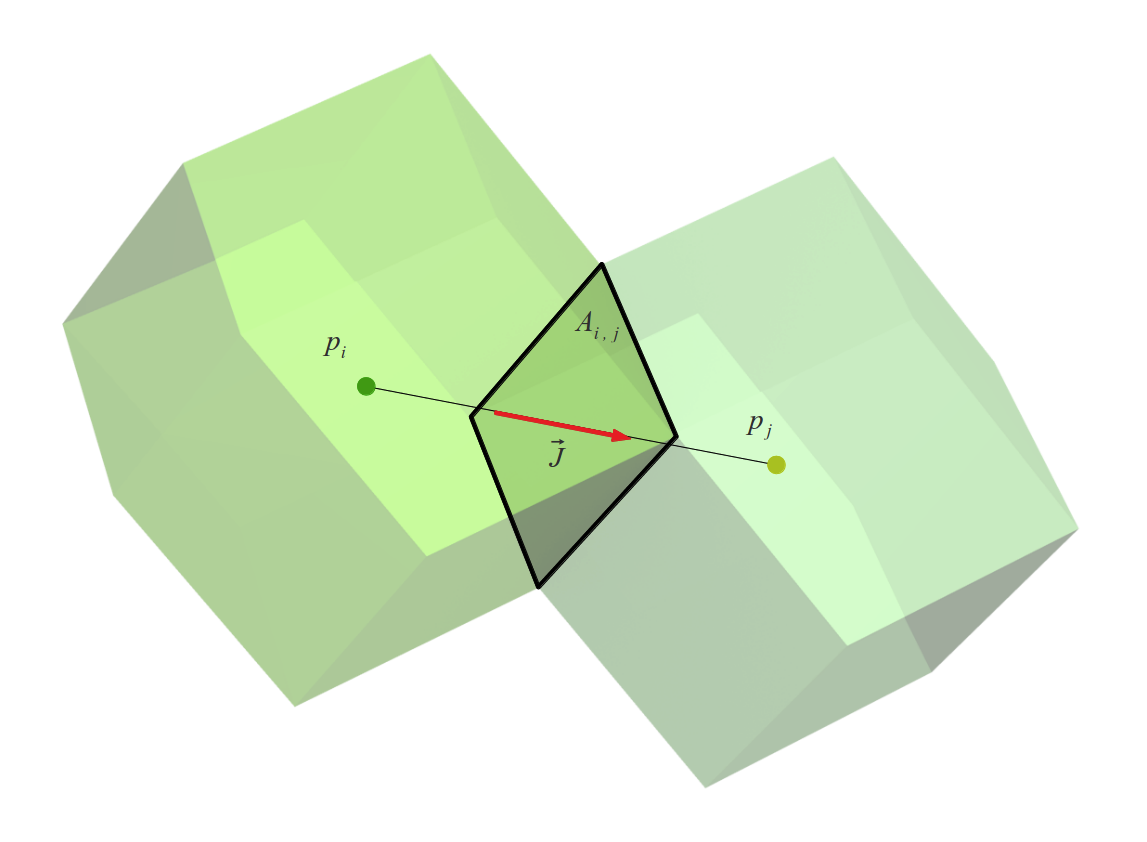
\includegraphics[width=0.8\textwidth]{../../images/model_grns/diffuse_volume_augmented_crop.png}
\end{center}
\caption{xx}
\label{model_grns_diffusion_schematic}
\end{figure}

The temporal evolution of the concentration is determined by the \textit{continuity equation}, which is a local form of conservation law. The divergence theorem gives the integral form of the continuity equation, applied on the volume of the cell. Its continuous expression reads:

$$\frac{\partial q_a}{\partial t} +  \iint_O \vec{J_a}.\vec{dA} = s_a + d_a $$

where $\vec{dA}$ is the normal vector of the closed surface of the cell, $s_a$ is the "source" term corresponding to the rate of ligand produced by secretion, and $d_a$ is the "sink" term corresponding to the rate of extracellular ligand $Q_a$ disappearing by the transduction activity of the cell. Finally, the discrete approximation of this closed surface integral is based on the topological neighbor list $\mathcal{N}^t_a$ (defined in Section 3.2.2) as follows:

$$\begin{eqnarray}        \frac{\partial q_{a,i}}{\partial t} & = & -\left(\sum_{j \in \mathcal{N}^t_a} \left\|\vec{J}_{a,ij}\right\| A_{i,j}\right) + s_{a,i} + d_{a,i} \\                & = & -D_a \left(\sum_{j \in \mathcal{N}^t_a} \frac{A_{ij}}{r_{ij}}(q_{a,j} - q_{a,i})\right) + \sigma_a p_{a,i} - \epsilon_a \tau_a' q_{a,i}      \end{eqnarray}$$
%  ====================================================================== 


\subsection{Illustration on Artificial GRN Motifs}
%  ====================================================================== 


  This section aims at offering a glimpse of the possibilities of our model of molecular and genetic regulation and signaling through simple idealized examples. E.H. Davidson's paper "Emerging properties of animal gene regulatory networks" \cite{Davidson:2010ez} offers various small GRN circuits that have been demonstrated to be involved in embryonic development.  

\subparagraph{Double negative gate}

  The first example introduces a sub-circuit called the \textit{double negative gate} which is part of the sea urchin embryo GRN \cite{Peter:2009dl}\cite{Davidson:2009gx}. The circuit allows the activation of a series of genes in a specific region of the embryo under the control of a localized expression (protein X in our example). The originality of the circuit is that X does not simply activate the series of downregulated genes (Target_1 and Target_2) but rather inhibits an inhibitor of these genes (Repressor_1 and Repressor_2) (Fig. XXXXX). This circuit aims at expressing the target genes in a particular domain, and shut them down in every other region of the embryo. 
\begin{figure}
\begin{center}
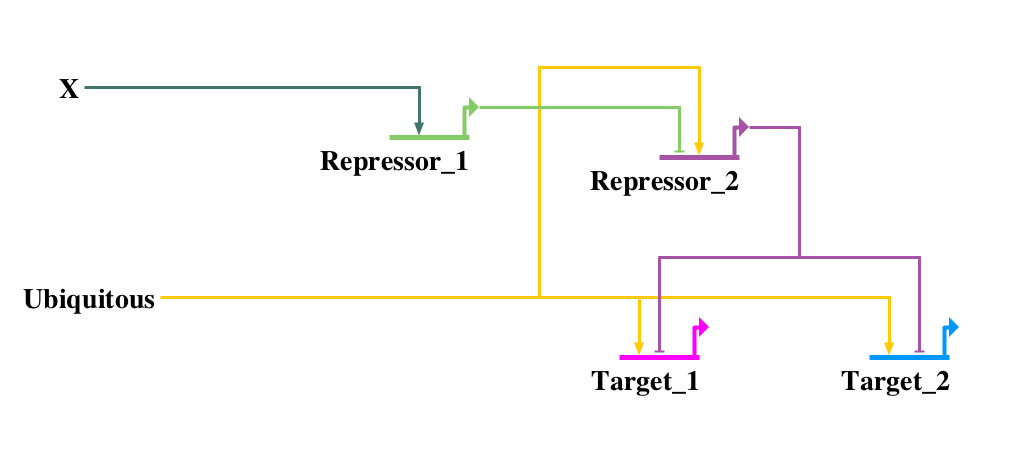
\includegraphics[width=0.9\textwidth]{../../images/Cases_Studies/Case_theo_grn/double_negative_gate/dng_grn.png}
\end{center}
\caption{\textbf{Double negative gate as displayed by the BioTapestry software from the file which inputs our model in this experiment.}}
\label{double_negative_gate_dng_grn}
\end{figure}

  We model this motif in a cell population comprising 4886 laid on a two cell deep planar configuration. The cells are immobile as they are in an equilibrium state and no active forces are exerted in between them. At the beginning, an ubiquitous protein (Ubiquitous) is activating both target genes Target_1 and Target_2, and their repressor Repressor_2 so that only the Repressor_2 encoded protein is expressed ubiquitously. At some point, the localized protein X is introduced in a part of the cell population (the protein concentration is artificially increased by adding the protein in those cells at a constant rate 0.1 unit per time step). In this example, all proteins have a similar degradation rate of 0.99 unit per time step so that the concentration of X tends toward an equilibrium quantity of 10 unit. As soon as the X concentration exceeds the threshold $\theta_{\mathrm{X},\mathrm{Repressor\_1}}$ of concentration of the cis-regulatory element of the target gene Repressor_1 ($\theta_{\mathrm{X},\mathrm{Repressor\_1}} = 1$), the protein of Repressor_1 starts to be produced at a rate 0.1 unit per time step. Once the concentration of protein Repressor_1 exceeds the threshold on the cis-regulatory element of Repressor_2 ($\theta_{\mathrm{Repressor_1},\mathrm{Repressor\_2}} = 9$), the gene state of Repressor_2 turns to value 0 as the boolean function relating both transcription factors Repressor_1 and Ubiquitous is a AND operator. Finally, the protein Repressor_2, which is not produced by its encoding gene any more, decreased in concentration by the molecular degradation mechanism. Once Repressor_2 concentration passes below the concentration threshold on its target genes Target_1 and Target_2 ($\theta_{\mathrm{Repressor\_2},\mathrm{Target\_1}} = 9$ and $\theta_{\mathrm{Repressor\_2},\mathrm{Target\_2}} = 9$) and as the boolean logic of both Target_1 and Target_2 is an AND operator, the target genes start being expressed in the region of the X protein. The time evolution of all proteins involved in region of X is shown in Fig. \ref{double_negative_gate_dng_grn_plot2} and a spatial visualization is shown in Fig. \ref{double_negative_gate_double_negative_gate_spatial}. 
\begin{figure}
\begin{center}
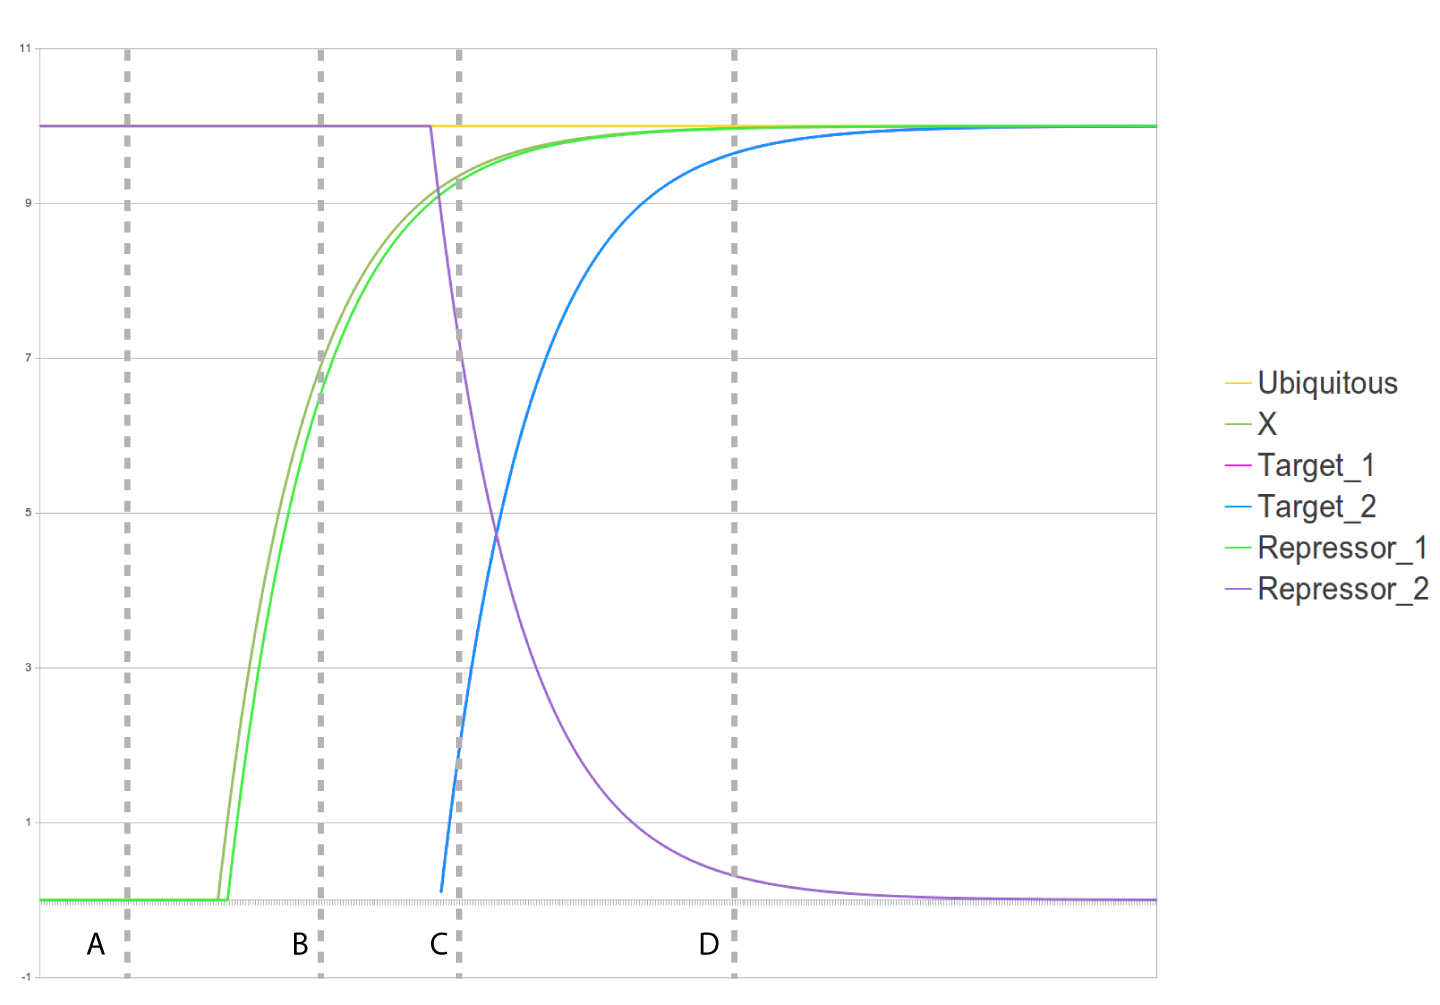
\includegraphics[width=0.9\textwidth]{../../images/Cases_Studies/Case_theo_grn/double_negative_gate/double_negative_gate_plot2_letter.png}
\end{center}
\caption{\textbf{Evolution of the proteins concentration in the region where X is expressed.} See text for the explanation of the curves' profile. The lettered bars indicate the timing of the snapshot shown in Fig. \ref{double_negative_gate_double_negative_gate_spatial}}
\label{double_negative_gate_dng_grn_plot2}
\end{figure}
\begin{figure}
\begin{center}
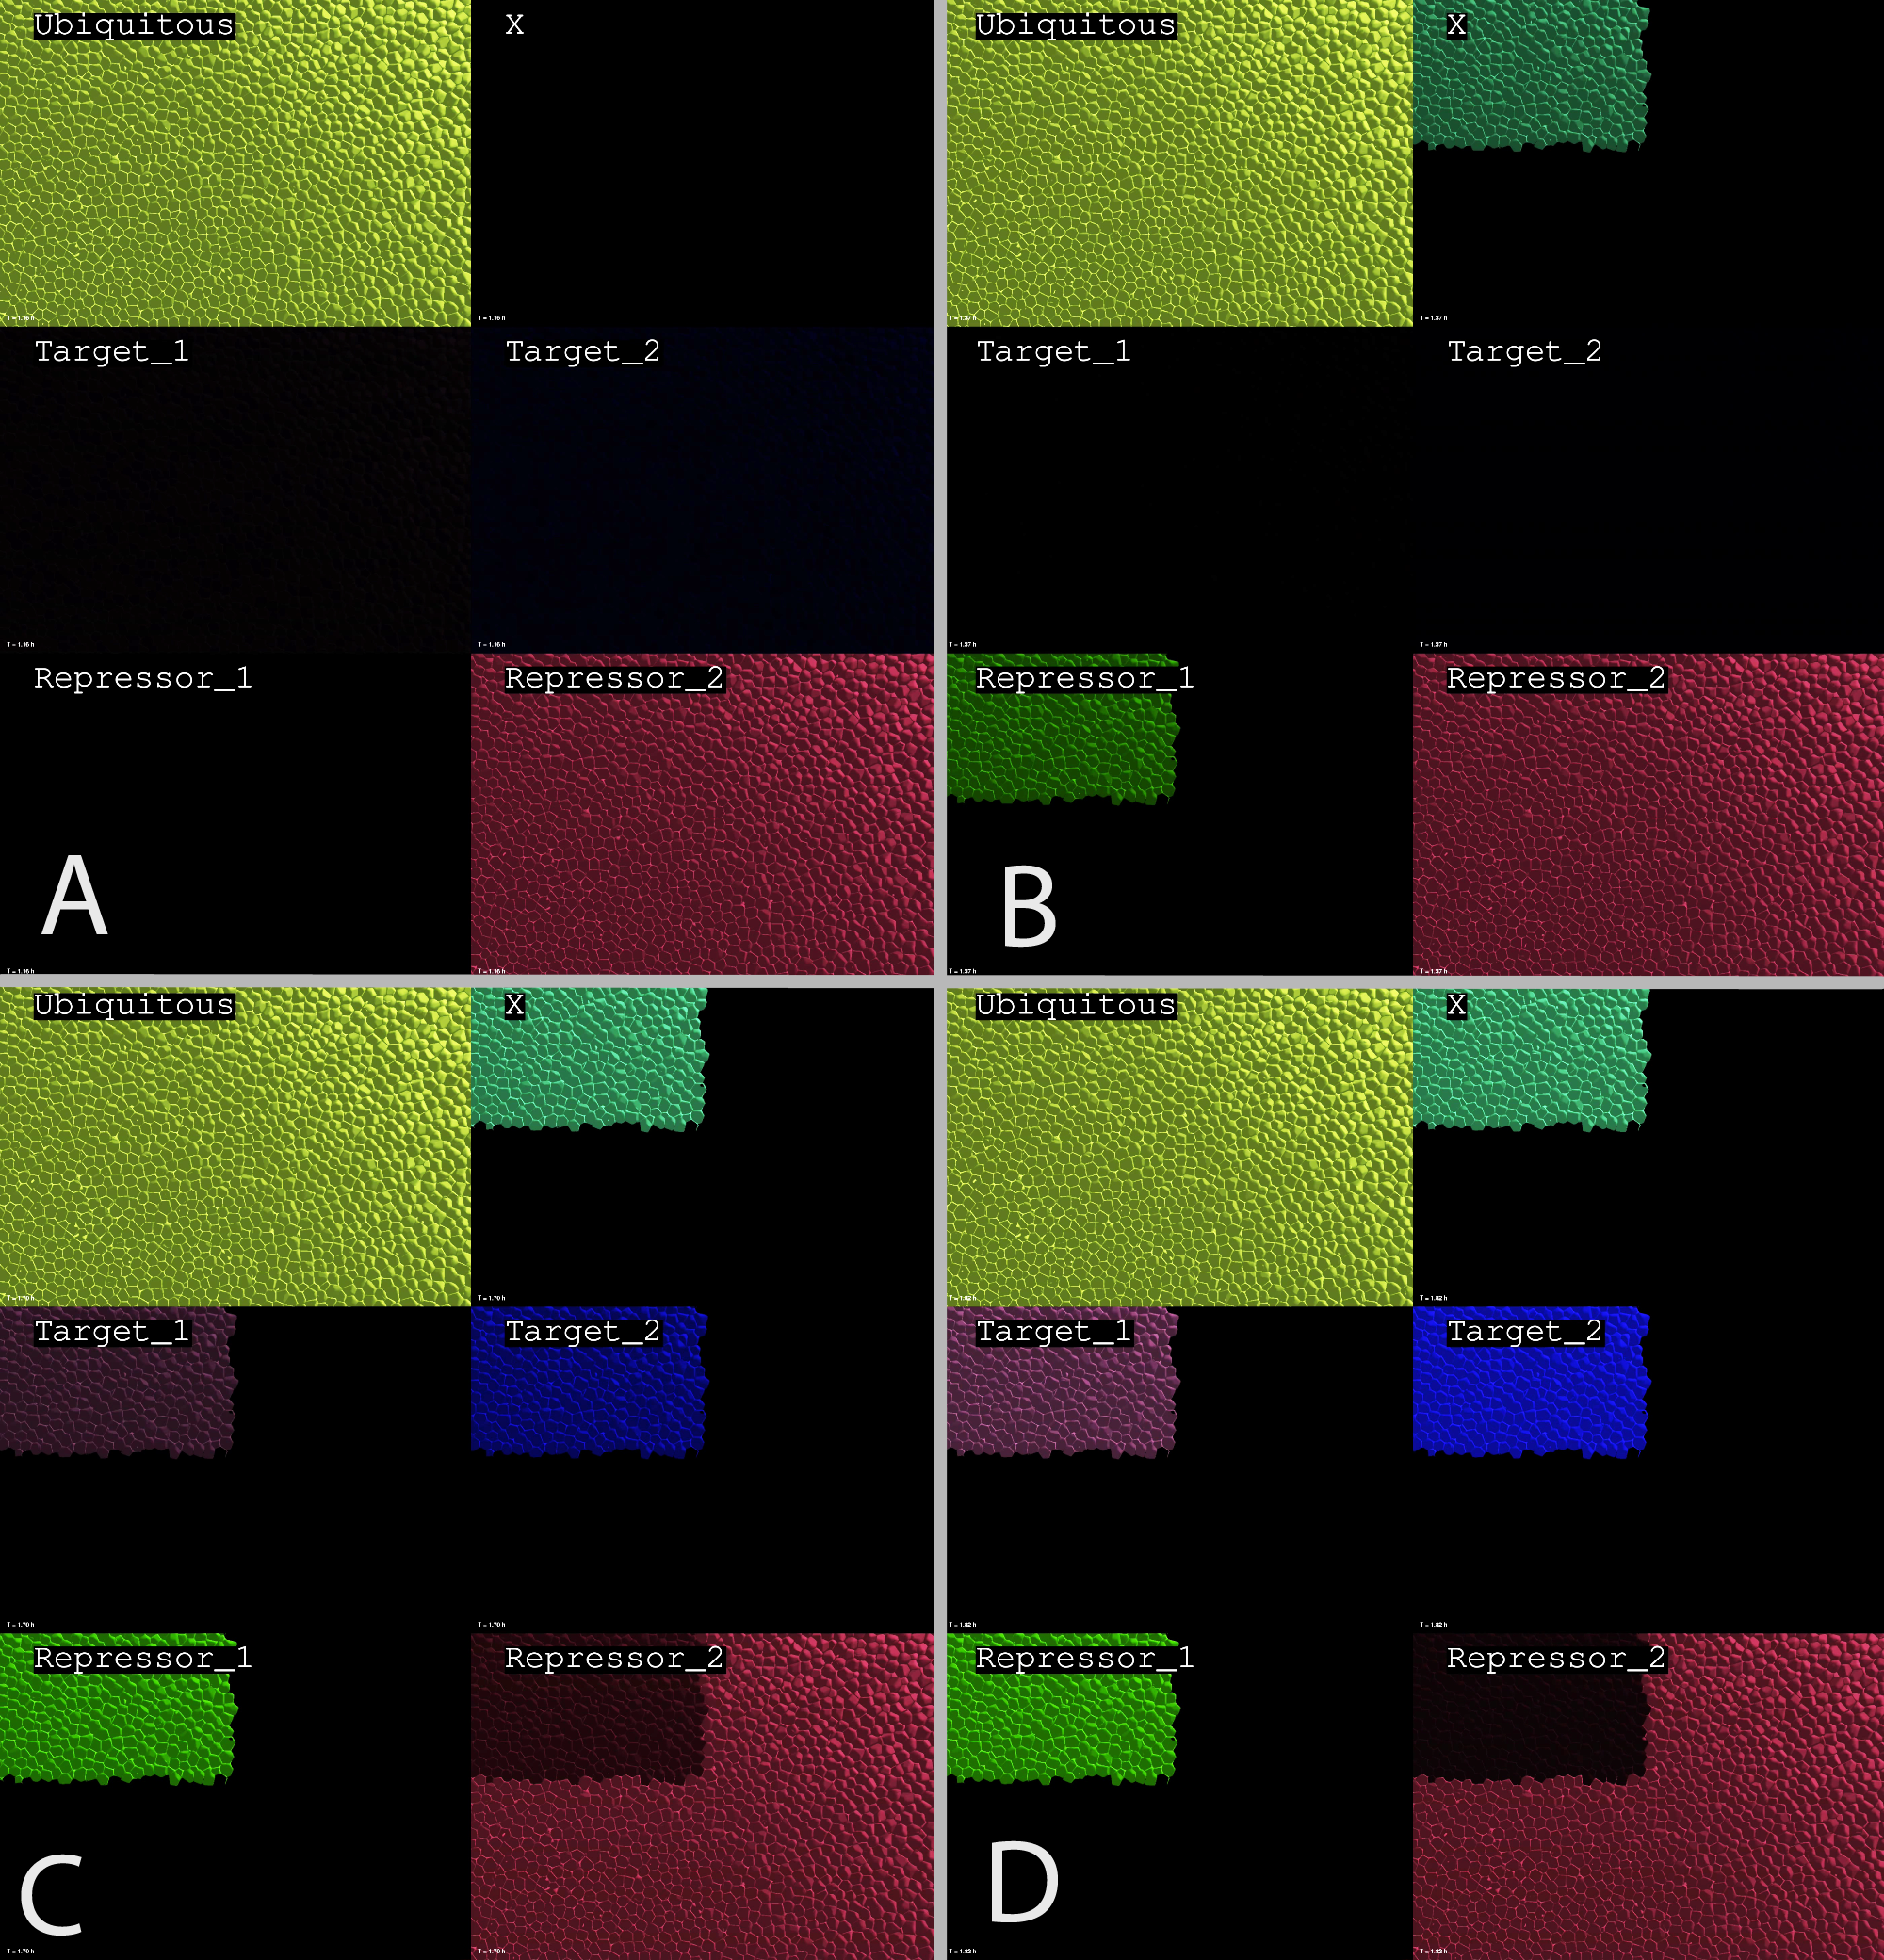
\includegraphics[width=0.9\textwidth]{../../images/Cases_Studies/Case_theo_grn/double_negative_gate/double_negative_gate_spatial.png}
\end{center}
\caption{\textbf{Spatial evolution of the protein concentration in the double negative gate experiment.} The letters correspond to the ones shown in Fig. \ref{double_negative_gate_dng_grn_plot2}. Each image is composed of 6 simultaneous views of the simulated cell population. The colors gives the concentrations of the proteins. The top left corner of each image is the region where the protein X is artificially secreted.}
\label{double_negative_gate_double_negative_gate_spatial}
\end{figure}

